\hyphenation{
For-schungs-pro-je-kte
For-schungs-vor-ha-ben}

\chapter{Einleitung}
	\abschnittsautor{F. Schäfer, M. Trognitz}

Für die Durchführung archäologischer und altertumswissenschaftlicher Forschungsprojekte ist die Anwendung von Informationstechnologien verschiedener Art immer geläufiger und selbstverständlicher. Dennoch fehlt es bis­lang an etablierten Strukturen, Standards und Verfahrensweisen, die allen Projekten den erprobten und effizienten Einsatz von IT ermöglichen, Vergleichbarkeit gewonnener Datenbestände erlauben, übergreifend gleichwertige Qualität digitalen Materials sicherstellen und die langfristige Les- und Nutzbarkeit von Forschungsergebnissen in digitaler Form garantieren. Durch die Einhaltung von Standards können nicht nur redundante Entwicklungsarbeiten mit zusätzlichen Finanzierungs-, Zeit- und Arbeitsaufwänden vermieden werden, sondern auch der Austausch von wissenschaftlichen Inhalten vereinfacht werden.

In zunehmendem Maße fordern auch wissenschaftspolitische Gremien, wie DFG, Wissenschaftsrat\footnote{\url{http://www.wissenschaftsrat.de/download/archiv/2359-12.pdf}} oder Schwerpunktinitiative "`Digitale Informationen"'\footnote{\url{http://www.allianzinitiative.de/de/handlungsfelder/forschungsdaten/grundsaetze}}, die Nachhaltigkeit und die Vernetzbarkeit digitaler wissenschaftlicher Informationen ein, was eine Auseinandersetzung mit Dateiformaten, Datenmanagement, Normen, Mindeststandards, semantischen Referenzmodellen, Dokumentations- und Austauschverfahren erforderlich macht -- sowohl bei kleineren Projekten eines Einzelnen als auch bei größeren disziplinen- und institutionenübergreifenden Forschungen. Einheitliche und in den jeweiligen Fachcommunities abgestimmte Vorgehen eröffnen für die aktuelle und zukünftige Forschung neue Möglichkeiten, um auf einer größeren, qualitätvolleren und homogeneren Datengrundlage komplexe Fragestellungen besser als bisher beantworten zu können.

Die IT-Empfehlungen sind als Hilfestellungen für alle Akteure in den Altertumswissenschaften konzipiert, um die langfristige Erhaltung und Benutzbarkeit des wissenschaftlichen Quellenmaterials zu gewährleisten sowie die Interoperabilität von Daten unterschiedlichen Ursprungs zu verbessern. Durch die Veröffentlichung von vollständigen digitalen Datensammlungen kann der Prozess der traditionellen Publikation von Forschungsergebnisse befördert und ergänzt werden, bspw. durch die zusätzliche Online-Bereitstellung von nicht in Druckform publizierten Katalogen, Analyseserien, Rekonstruktionen o. ä. m. (sog. Datenpublikationen).

Die hier zusammengetragenen IT-Empfehlungen befassen sich vor allem mit der Frage, wie digitale Daten besser ausgetauscht, für die Zukunft aufbewahrt und dauerhaft verstanden werden können. Sie fokussieren also auf technische Formate und inhaltliche Beschreibung von Daten und Methoden, die für die langfristige Archivierung, Bereitstellung und Nachnutzung von Daten von zentraler Bedeutung sind. Spezifische Vorgaben zu fachlichen Methoden, Fragestellungen, Workflows oder Anwendungen sind dagegen nicht Gegenstand der Empfehlungen.

Weitere Informationen zur Relevanz und Kuratierung von digitalen Forschungsdaten in den Altertumswissenschaften sind in den "`Guides to Good Practice"'\footnote{\url{http://guides.archaeologydataservice.ac.uk/g2gp/GuideAim}} des Archaeology Data Service zu finden, wo ebenfalls auf weiterführende Publikationen verwiesen wird. 


\section*{Umsetzung}
In der Regel wird es in bestimmten Phasen eines Projektes oder aufgrund institutioneller Rahmenbedingungen notwendig sein, von diesen IT-Empfehlungen abzuweichen, vor allem während der Generierung und der Auswertung von Daten. Da im Folgenden nur minimale Standards beschrieben werden, kann es für deren praktische Anwendung hilfreich sein, darüber hinausgehende Spezifizierungen festzulegen, z. B. Wege zur konkreten Umsetzung von Vorgaben zu definieren, Zuständigkeiten beim Forschungsdatenmanagement zu verteilen oder zusätzliche forschungs- bzw. organisationsspezifische Bedingungen zu diskutieren. Diese Spezifizierungen sowie Abweichungen von Standards sollten immer sorgfältig abgewogen, hinsichtlich der digitalen Nachhaltigkeit und Austauschbarkeit hinterfragt und ausreichend dokumentiert werden. Zudem gilt es jeweils zu prüfen, ob dadurch zusätzliche Arbeitsschritte erforderlich werden.

Da Forschungsdaten in hohem Maße von einem zyklischen Charakter geprägt werden, wie beim Lebenszyklus von Daten auf Seite \pageref{lebenszyklus} beschrieben, sind die Archivierung und Nachnutzung von Daten keine Aspekte, die erst am Ende eines Projektes zu behandeln sind, sondern bereits vor bzw. bei der Erhebung der ersten digitalen Dateien berücksichtigt werden müssen.

Wird z. B. bei Fotografien nicht von Anfang an festgehalten, wer an welchem Ort und zu welchem Zeitpunkt ein Bild aufgenommen hat, oder bei Messungen gerätespezifische Eigenschaften, die die Qualität von Daten bestimmen, nicht dokumentiert, so können diese wichtigen Angaben nach dem Projektende fehlen oder mangels Personal, Finanzmittel oder Möglichkeiten nachträglich nicht mehr erhoben werden. Forschungsdaten sind dadurch potentiell in ihrer Qualität für eine wissenschaftliche Nachnutzung durch Dritte stark eingeschränkt. Ähnlich kann es sich bei der Verwendung proprietärer Formate verhalten, bei denen einerseits eine Migration auf neuere Programmversionen nur mit inhaltlichen und/oder funktionalen Verlusten einhergeht und andererseits kein Export der Inhalte in anwendungsunabhängige Formate unterstützt wird. In diesem Fall ist ein realer Datenverlust vorhersehbar.

Zur Verwirklichung der hier aufgeführten IT-Empfehlungen sollten Einrichtungen entsprechende Strukturen aufbauen, die Forschungsprojekte bei der Formulierung von IT-Konzepten beraten und diese begutachten, die bei der Implementierung eines Forschungsdatenmanagements unterstützen, die die Qualitätskontrolle von Daten übernehmen sowie deren langfristige Verfügbarkeit und Archivierung gewährleisten.

Für laufende Projekte und "`Altdaten"' gilt Bestandsschutz. Da aber auch diesen Daten ein hoher wissenschaftlicher Wert zukommt, den es in der Regel zu erhalten gilt, ist auch hier eine Anpassung bzw. Migration auf aktuelle Standards und Empfehlungen in jedem Fall erstrebenswert und es sollte immer geprüft werden, ob ein solcher Schritt möglich ist.

Weiterhin ist der Einsatz von Informationstechnologien und der Umgang mit digitalen Daten an die Berücksichtigung des Urheberrechts und des Datenschutzes gebunden.


\subsection*{Wann sollten Sie diese Empfehlungen berücksichtigen?}
\begin{itemize}
	\item In der Antrags- und Planungsphase eines neuen Projektes, um frühzeitig technische, personelle und finanzielle Anforderungen und Lösungen berücksichtigen zu können
	\item Während der Durchführung von Forschungsprojekten als Referenz für spezifische Fragen und Probleme
	\item Vor der Übergabe von Daten an ein institutionelles Archiv oder Datenrepositorium
\end{itemize}

\subsection*{Autoren und Quellen der Empfehlungen}
Die hier präsentierten Empfehlungen und Hintergrundinformationen beruhen im Wesentlichen auf drei Quellen.

1. \textbf{Texte von Fachspezialisten}, die aus unterschiedlichen Institutionen, Disziplinen und Projekten stammen und Vorschläge für die jeweiligen Fachcommunities formuliert haben. Entsprechend werden am Ende der einzelnen Kapitel die maßgeblichen Autoren genannt. Dieser Prozess wurde seit 2007 von der Deutschen Forschungsgemeinschaft angestoßen und unterstützt (u. a. durch die Finanzierung vorbereitender Arbeitstreffen) sowie durch das Deutsche Archäologische Institut in seiner Gesamtheit koordiniert. IANUS hat für die Ergebnisse die technische Plattform bereitgestellt und die redaktionelle Qualitätssicherung übernommen. Die weitere Pflege und Aktualisierung der IT-Empfehlungen wird durch entsprechende Mitarbeiter übernommen sowie ihre Umsetzung durch entsprechende Angebote unterstützt.

2. Der vom DAI entwickelte \href{http://www.ianus-fdz.de/it-empfehlungen/downloads\#dai-leitfaden}{"Leitfaden zur Anwendung von Informationstechniken der archäologischen Forschung"}\footnote{\url{http://www.ianus-fdz.de/it-empfehlungen/downloads\#dai-leitfaden}}, der sich im Downloadbereich befindet, wird vollständig durch die von IANUS betreuten IT-Empfehlungen abgelöst. Inhalte dieses IT-Leitfadens sind vollumfänglich in die hier formulierten Mindeststandards eingeflossen und wo notwendig aktualisiert bzw. ergänzt worden.

3. \textbf{Standards und Veröffentlichungen anderer Einrichtungen}, um die hier formulierten Mindeststandards in den nationalen und internationalen Kontext zu stellen und länderübergreifende Übereinstimmung in Kernfragen zu erreichen. Hervorzuheben sind in diesem Kontext besonders die \href{http://guides.archaeologydataservice.ac.uk/g2gp/Main}{"Guides to Good Practice"}\footnote{\url{http://guides.archaeologydataservice.ac.uk/g2gp/Main}} des Archaeology Data Service in York, England und der Digital Antiquity in Tempe, Arizona, USA, die \href{http://www.dcc.ac.uk/resources/how-guides}{"How-to Guides"}\footnote{\url{http://www.dcc.ac.uk/resources/how-guides}} des Digital Curation Center in London, England und der noch nicht finalisierte \href{http://www.landesarchaeologen.de/fileadmin/Dokumente/Dokumente_Kommissionen/Dokumente_Archaeologie-Informationssysteme/Dokumente_AIS_Archivierung/Ratgeber-Archivierung_Vorab-V0.07.pdf}{"Ratgeber zur Archivierung Digitaler Daten"}\footnote{\url{http://www.landesarchaeologen.de/fileadmin/Dokumente/Dokumente_Kommissionen/Dokumente_Archaeologie-Informationssysteme/Dokumente_AIS_Archivierung/Ratgeber-Archivierung_Vorab-V0.07.pdf}} des Verbandes der Landesarchäologen in Deutschland.

%##################################################################
%##################################################################
%##################################################################
\newpage
\section{Benutzung der IT-Empfehlungen}
\abschnittsautor{F. Schäfer, M. Trognitz}
Die IT-Empfehlungen für den nachhaltigen Umgang mit digitalen Daten in den Altertumswissenschaften liegen sowohl in statischer Form als verschiedene PDF-Dateien vor, als auch in dynamischer Form auf \href{https://www.ianus-fdz.de/it-empfehlungen}{www.ianus-fdz.de/it-empfehlungen}. Beide Formen sind inhaltlich identisch und können unabhängig voneinander verwendet werden. Die Webseite bietet neben vielfältigen Verlinkungen und Downloads weitere Funktionalitäten, zu denen auch eine Suchfunktion und ein integriertes Glossar gehören. Die PDF-Dokumente eignen sich dagegen z. B. als Hilfsmittel im Feld, das individuell ausgedruckt werden kann.

Die IT-Empfehlungen umfassen neben diesem Einleitungskapitel die drei Kapitel \textbf{Projektphasen}, \textbf{Datenformate} und \textbf{Forschungsmethoden}.

\subsection*{Aufbau der einzelnen Kapitel}
In dem Kapitel \textbf{Projektphasen} sind allgemeine Hinweise hinterlegt, die sich mit den konkreten Arbeitweisen und Phasen in Forschungsprojekten befassen. Es enthält Hinweise darauf, was bei der Planung und dem Beginn eines Projektes zu beachten ist, welche Aspekte während der Projektdurchführung, also vor allem bei der Erhebung und Verwaltung von Forschungsdaten, wichtig sind und welche Fragen beim Abschluss eines Forschungsvorhabens beantwortet werden sollten. 

Das Kapitel \textbf{Dateiformate} beinhaltet einerseits konkrete Hinweise zu den technischen Dateiformaten, die nach heutigem Wissen für die Langzeitarchivierung geeignet sind. Andererseits werden die minimalen Anforderungen an die Dokumentation von Forschungsdaten genannt, damit diese nicht nur heute, sondern auch in Zukunft von Dritten verstanden und nachgenutzt werden können. Diese Abschnitte sind weiter unterteilt in: \textbf{Übersicht}, \textbf{Vertiefung}, \textbf{Praxis} und \textbf{Quellen}.

Der Unterabschnitt \textbf{Übersicht} bietet eine Zusammenfassung über die jeweils geeigneten technischen Formate, die erforderlichen Metadaten und eventuelle Fehlerquellen. Er richtet sich sowohl an den erfahrenen Anwender als auch an Nutzer mit konkreten, schnell zu beantwortenden Fragen. Die Informationen aus allen Übersichts-Abschnitten werden in einer eigenen PDF-Datei als Kurzfassung der IT-Empfehlung zusammengefasst und zum Download bereit gestellt. Zu beachten ist, dass die angegebenen Metadaten nur ein Minimum darstellen und gegebenfalls abhängig vom Projektkontext und der verwendeten Methode ergänzt werden müssen.

Der interessierte Nutzer findet im Unterabschnitt \textbf{Vertiefung} weiterführende Hintergrundinformationen über die in der jeweiligen Übersicht angesprochenen Teilaspekte und im Abschnitt \textbf{Praxis} werden praktische Anleitungen, Vorlagen, Formulare, Best-Practice-Beispiele und andere nützliche Werkzeuge gesammelt, die bei der praktischen Umsetzung der beschriebenen Mindeststandards helfen sollen. Ergänzende Informationen werden in dem Unterabschnitt \textbf{Quellen} gelistet.

Das Kapitel \textbf{Forschungsmethoden} befasst sich mit den verschiedenen in den Altertumswissenschaften angewandten Methoden und Disziplinen. Auch wenn langfristig eine möglichst hohe Vollständigkeit angestrebt wird, ist es nicht Ziel und Zweck der IT-Empfehlungen, ein umfassendes Handbuch über die Geschichte, Fragestellungen, Anwendung oder Vor-/Nachteile aller relevanten Methoden und Arbeitsweisen zu sein. Stattdessen stehen Dokumentation und Metadaten im Vordergrund, die für das Verständnis, die Nachvollziehbarkeit und Nachnutzbarkeit der generierten digitalen Daten durch Dritte zentral sind. Wie bei den Dateiformaten sind auch hier die einzelnen Abschnitte in \textbf{Übersicht}, \textbf{Vertiefung}, \textbf{Praxis} und \textbf{Quellen} untergliedert. Sofern bei einzelnen Disziplinen spezifische Dateiformate eine besondere Relevanz besitzen, sind diese entweder hier beschrieben oder es wird mittels Links auf die entsprechenden Abschnitte im Kapitel "`Dateiformate"' verwiesen.

Häufig genutzte oder zentrale Fachbegriffe werden in einem \textbf{Glossar} erklärt und sind auf der Webseite unterstrichen. Wenn der Mauszeiger auf einem markierten Wort liegt, wird die Erklärung mittels Tooltip eingeblendet.

Im \textbf{Download-Bereich} können sowohl die verschiedenen längeren und kürzeren Varianten der aktuellen IT-Empfehlungen als auch älteren Versionen heruntergeladen werden. Außerdem sind hier zentrale Dokumente für die Archivierung von Forschungsdaten in IANUS enthalten. 

In der \textbf{rechten Spalte} findet man Materialien zum Download, die auf den gerade ausgewählten Abschnitt abgestimmt sind.

\subsection*{Zitation der IT-Empfehlungen}
Die gesamten IT-Empfehlungen können als eine einzige Publikation betrachtet werden, deren unterschiedliche Kapitel von unterschiedlichen Autoren verfasst wurden. Auf die einzelnen Kapitel kann unter Nennung der Autoren entweder auf die Online-Version oder auf die Vollversion als PDF-Dokument verwiesen werden:
\begin{itemize}
	\item M. Trognitz -- P. Grunwald, Bilder -- Rastergrafiken, in: IANUS (Hrsg.), IT-Empfehlungen für den nachhaltigen Umgang mit digitalen Daten in den Altertumswissenschaften (25.01.2017) [online] doi: \url{http://dx.doi.org/10.13149/000.111000-a}
	\item M. Trognitz -- P. Grunwald, Bilder -- Rastergrafiken, in: IANUS (Hrsg.), IT-Empfehlungen für den nachhaltigen Umgang mit digitalen Daten in den Altertumswissenschaften (2017) [Version 1.0.0.0] doi: \url{http://dx.doi.org/10.13149/000.y47clt-t}
\end{itemize}

Die  Online-Version der IT-Empfehlungen ist immer die aktuellste Fassung und hat für die dauerhafte Referenzierung einen DOI:

\begin{itemize}
	\item IANUS (Hrsg.), IT-Empfehlungen für den nachhaltigen Umgang mit digitalen Daten in den Altertumswissenschaften (Abrufdatum) [online] doi: \url{http://dx.doi.org/10.13149/000.111000-a}
\end{itemize}

Für die PDF-Version muss zusätzlich die Versionsnummer angegeben werden, da diese von Zeit zu Zeit aktualisiert und als Download zur Verfügung gestellt werden. Die Versionsnummer besteht aus vier Stellen, die Auskunft über die verschiedenen Änderungen geben:

\begin{center}
	\Large \bfseries Version 1.0.0.0
\end{center}

Die erste Stelle ändert sich nur, wenn grundlegende Veränderungen an den IT-Empfehlungen vorgenommen werden. Die zweite Stelle ändert sich, sobald ein neues Kapitel hinzukommt. Wenn sich die zweite Stelle ändert, bekommt das jeweilige PDF einen neuen DOI. Die dritte Stelle erhöht sich, sobald an den Formatempfehlungen oder in anderen Abschnitten Änderungen mit substantiellen Auswirkungen auf die konkrete Datenpraxis vorgenommen werden. Alle weiteren Änderungen, wie Korrekturen, kleinere Ergänzungen im Text oder Ergänzungen im Glossar, werden mit der vierten Stelle der Versionsnummer gekennzeichnet. Eine Tabelle am Beginn des PDF-Dokumentes gibt Auskunft über die Art der jeweiligen Änderungen.

Beispielsweise wird Version 1.2.0.0 im Vergleich zu Version 1.0.0.0 mindestens zwei neue Kapitel enthalten. Version 1.0.1.0 wird im Vergleich zu 1.0.0.0 Änderungen an den empfohlenen Langzeitformaten oder umfängliche andere Änderungen enthalten. Für die praktische Verwendung sind Version 1.0.1.0 und Version 1.0.1.5 gleichermaßen geeignet, da sie die gleichen Empfehlungen für Langzeitformate enthalten und sich lediglich in Korrekturen oder Ergänzungen unterscheiden. 

\subsection*{Mitarbeit und Diskussion}
Jeder Abschnitt in den Kapiteln \textbf{Dateiformate} und \textbf{Forschungsmethoden} enthält einen Unterabschnitt \textbf{Diskussion}, der angemeldeten Nutzern die Möglichkeit bietet, Hinweise und Kommentare, z. B. zu nützlichen Softwaretools oder neuen Standards, zu hinterlegen. Ebenso können hier noch fehlende oder unzureichend formulierte Aspekte benannt werden oder gemachte Empfehlungen offen diskutiert werden. Daneben kann natürlich auch eine E-Mail an it-empfehlungen.ianus-fdz@dainst.de geschickt werden, um individuelle Anmerkungen zu formulieren oder die Bereitschaft zur Mitarbeit bei neuen oder zu aktualisierenden Kapiteln zu signalisieren. Alle Rückmeldungen werden regelmäßig von Mitarbeitern in IANUS geprüft und gegebenfalls in die IT-Empfehlungen eingearbeitet. 

%##################################################################
%##################################################################
%##################################################################
\newpage
\section{Der Lebenszyklus von Forschungsdaten}
\label{lebenszyklus}
\abschnittsautor{M. Trognitz}
Die Anforderungen an das Management von Forschungsdaten gehen weit über die Langzeitarchivierung, einer Kernaufgabe von IANUS, hinaus. Daher soll im Folgenden kurz auf das Konzept des Datenlebenszyklus eingegangen werden. 

Forschungsdaten haben im Allgemeinen eine deutlich längere Lebensdauer als die Projekte, in denen sie entstanden sind. Auch nach Ablauf von Förderungsphasen kann es sein, dass Forscher weiterhin an den Daten arbeiten oder sie werden in Folgeprojekten weiter verarbeitet und ergänzt. Die Daten können auch von anderen Wissenschaftlern unter Berücksichtigung neuer Forschungsfragen wiederverwendet werden. Somit können aus bereits gesammelten Forschungsdaten neue Daten entstehen. Dieser Kreislauf wird mit dem sogenannten Datenlebenszyklus beschrieben. 

\begin{wrapfigure}{r}{0.51\textwidth}%0.51
  \begin{center}
    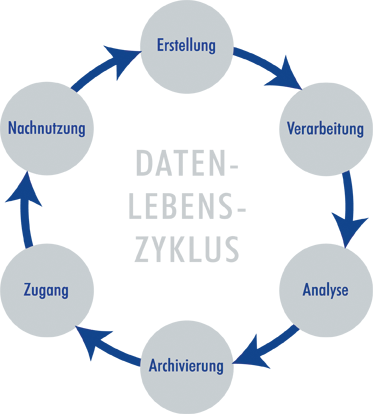
\includegraphics[width=0.51\textwidth]{bilder/Datenlebenszyklus}
  \end{center}
  \caption{Datenlebenszyklus}
\end{wrapfigure}

In der gegenwärtigen Praxis ist der Datenlebenszyklus oft unterbrochen, da nur einige wenige Daten ihren Weg in eine Publikation finden. Die übrigen Daten geraten auf den lokalen Speichermedien der Forscher in Vergessenheit oder werden komplett gelöscht und stehen somit einer Nachnutzung nicht mehr zur Verfügung. Diese Tatsache gilt es für die Zukunft zu verbessern und im Idealfall vollständig zu vermeiden.

Der hier vorgestellte Datenlebenszyklus beruht auf dem des "`UK Data Archive"'\footnote{\url{http://data-archive.ac.uk/create-manage/life-cycle}}. Er beschreibt sehr vereinfacht und idealtypisch die Abfolge der einzelnen Phasen im Zyklus aus einem eher praktischen Umgang mit Forschungsdaten. Es gibt auch andere komplexere Modelle, die einen anderen Blickwinkel beschreiben, wie etwa das "`Curation Lifecycle Model"'\footnote{\url{http://www.dcc.ac.uk/resources/curation-lifecycle-model}}, das verschiedene Tätigkeitsfelder bei der Erhaltung und Pflege der Daten beschreibt, und das "`Data Curation Continuum"'\footnote{\url{http://www.dlib.org/dlib/september07/treloar/09treloar.html}}, das vor allem auf die technischen Bedingungen eingeht und Daten unter dem Gesichtspunkt der Nutzergruppen, von privat bis öffentlich, beschreibt.

In jeder Phase des Datenlebenszyklus gelten unterschiedliche Schwerpunkte mit ihren eigenen Implikationen, die im Folgenden umrissen werden. In dem Kapitel Projektphasen ab Seite \pageref{projektphasen} werden die wichtigsten Aspekte dann ausführlich behandelt.

\subparagraph{Erstellung} Vor der eigentlichen Erstellung von neuen Daten muss schon die Projektplanung erfolgt und die Fragestellung formuliert sein, die maßgeblich bestimmen, wie die gesammelten und erzeugten Daten letztendlich aussehen sollen. Ein Bestandteil der Planung muss auch das Datenmanagement sein, das ab Seite \pageref{datenmanagement} beschrieben wird, um vorab festzulegen, welche Formate und Benennungsregeln verwendet werden sollen, wie die Speicherung und Sicherung der Daten und die Vernetzung von Daten und Projektmitarbeitern untereinander aussehen soll. Bereits vorhandene relevante Daten sollten lokalisiert und berücksichtigt werden. 

Schon während der Erstellung der Forschungsdaten erfolgt idealerweise die Beschreibung der Daten, da diese besonders im Hinblick auf die spätere Nachnutzung für die Verständlichkeit eine elementare Rolle spielt. Beispielsweise müssen die technischen Parameter der verwendeten Aufnahmegeräte so früh wie möglich dokumentiert werden.

\subparagraph{Verarbeitung} Sobald die Daten erhoben wurden, können sie verarbeitet werden. Dazu gehören verschiedene Abläufe, wie etwa Digitalisierung, Übersetzung, Überprüfung, Validierung, Bereinigung und andere Verarbeitungsformen mittels Programmen. Für einige Anwendungen oder im Hinblick auf eine spätere Veröffentlichung, kann eine Anonymisierung notwendig sein. Auch gilt es festzuhalten, wie Ausgangsdaten verändert und bearbeitet wurden. 

Außerdem ist die Beschreibung von Forschungsdaten ein wichtiger Aspekt für die Archivierung, um die Verständlichkeit für die spätere Nachnutzung deutlich zu erhöhen. Während der Verarbeitung von Forschungsdaten spielt die Verwaltung und Speicherung der Daten eine große Rolle, da gewährleistet werden muss, dass mit der richtigen Version gearbeitet wird und notfalls auch Sicherheitskopien zur Verfügung stehen.

\subparagraph{Analyse} Durch die Analyse und Interpretation der Forschungsdaten werden die Forschungsergebnisse gewonnen, die dann in Publikationen veröffentlicht werden. In der Regel sind die den neuen Erkenntnissen zugrunde liegenden Daten aber nur ein kleiner Bestandteil einer solchen Publikation. Jedoch werden alle Daten benötigt, um die Analyseergebnisse vollständig nachvollziehen zu können.

\subparagraph{Archivierung} Die Archivierung von Forschungsdaten beinhaltet die Auswahl und Umwandlung der einzelnen Dateien in geeignete Formate und deren Speicherung auf einem für die Archivierung geeigneten Medium. Die Erstellung und Speicherung von Backups gehört ebenfalls dazu.

Eine wesentliche Rolle bei der Archivierung spielt sowohl die strukturierte als auch die freie Beschreibung der Forschungsdaten, da diese Informationen darüber enthalten, wie und durch wen die Daten gewonnen wurden, welche Geräte dabei Verwendung fanden, wie diese konfiguriert waren und was die Daten bedeuten. 

\subparagraph{Zugang} Da das Ziel einer Datenarchivierung immer die Nachnutzbarkeit von Inhalten ist, sollten archivierte Daten im Rahmen rechtlicher Rahmenbedingungen verbreitet und Dritten ein Zugriff auf diese gewährt werden. Den Zugriff auf die Daten kann man mit verschiedenen Zugriffsrechten steuern, die es beispielsweise nur einer eingeschränkten Gruppe von Nutzern erlauben auf die Daten zuzugreifen. Bevor die Daten zugänglich gemacht werden, sollte man dafür sorgen, dass das Urheberrecht geklärt und gekennzeichnet ist.

Durch die Zugriffsgewährung wird die Sichtbarkeit von eigenen Forschungsleistungen erhöht.

\subparagraph{Nachnutzung} Archivierte Daten, die zugänglich gemacht wurden, können für eigene Forschungsvorhaben kostenlos wiederverwendet und neuen Analysen unterzogen werden. Durch die Nachnutzung wird die Nachprüfbarkeit von Ergebnissen im Sinne der guten wissenschaftlichen Praxis erleichtert.